\label{sec:empirical}

\begin{figure}[t!]
\center
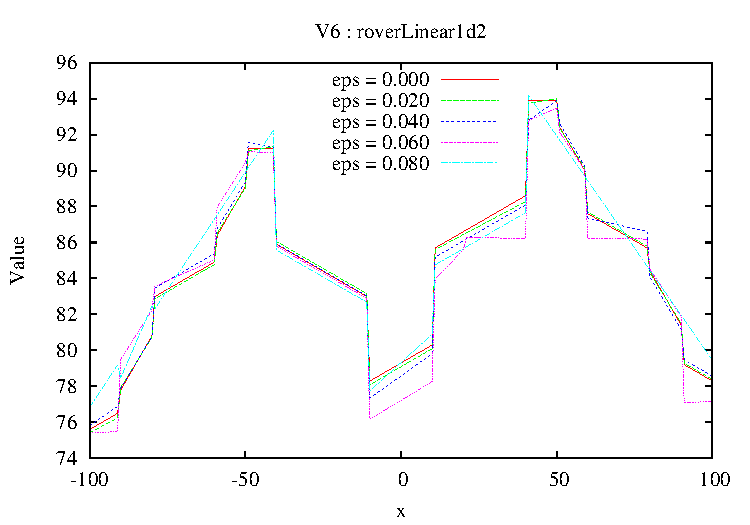
\includegraphics[width=0.48\textwidth]{Figures/rover1D/roverLinear1d2V6.pdf} 
\caption{\footnotesize Value function at iteration 6 for $\MarsRoverUni$, showing how different levels of approximation error (eps) lead to different compressions.}
\label{fig:rover1dv6} 
\end{figure}

In this section we wish to compare the scalability of exact SDP
(calling BASDP in Algorithm~\ref{sec:basdp} with $\epsilon=0$)
vs. various levels of approximation error $\epsilon > 0$ to determine
the trade-offs between time and space vs. approximation error.
To do this, we evaluated BASDP on three different domains ---
\MarsRoverUni, \MarsRoverBi and \Invent --- detailed next.

\MarsRoverUni:
This is a unidimensional continuous Mars Rover domain motivated by
Bresina {\it et al}~\cite{bresina02} used in order to visualize the
value function and the effects of varying levels of approximation.
The position of the rover is represented by a single continuous
variable ($x$) and the goal of the rover is to take pictures at
specific positions.  There is only one action $\mathit{move}(a_x)$,
where $a_x$ is the movement distance. In the description of the
problem for instance roverLinear1d2 shown below, there are two picture
points and taking pictures is recorded in two boolean variables
($tp_1$ and $tp_2$). The dynamics for action $move(a_x)$ is as
follows: {\footnotesize
\begin{align*}
tp_1' &= \begin{cases}
tp_1 \vee (x>40 \wedge x<60)&: 1\\
else&: 0\\
\end{cases}\\
tp_2' &= \begin{cases}
tp_2 \vee (x>-60 \wedge x<-40)&: 1\\
else&: 0\\
\end{cases}\\
x' &=  x +a_x\\
R & = R_1 + R_2 + R_3\\
R_1 & = \begin{cases} 
(tp_1') \wedge (\neg tp_1) \wedge (x > 50) &: 40 - 0.2*(x -50)\\
(tp_1') \wedge (\neg tp_1) \wedge (x < 50) &: 40 - 0.2*(50-x)\\
(tp_1') \wedge ( tp_1) &:  1.1\\
else &: -2\\
\end{cases} \\
R_2 & = \begin{cases} 
(tp_2') \wedge (\neg tp_2) \wedge (x > -50) &: 60 - 0.2*(-x +50)\\
(tp_2') \wedge (\neg tp_2) \wedge (x < -50) &: 60 - 0.2*(x +50)\\
(tp_2') \wedge ( tp_2) &:  1.2\\
else &: -1\\
\end{cases} \\
R_3 & = \begin{cases} 
a_x > 0 &: -0.1*a_x\\
a_x < 0 &: 0.1*a_x\\
\end{cases} \\
\end{align*} }
\vspace{-10mm}

In Figure~\ref{fig:rover1dv6}, we plot different value functions obtained by compressing with different levels --- in general we note that a larger $\epsilon$ results in a looser fit, but we note that there are some exceptions, owing to the greedy nature of successive pairwise merging for XADDs described in Section~\ref{sec:approx}.

\MarsRoverBi: In this multivariant version of a \MarsRover~domain there are no picture points but the rover is expected to follow a path. The position is represented by a pair or continuous variables $(x,y)$. There is only one action, $move(a_x,a_y)$, where $|a_x| < 10$ and $|a_y| < 10$. The new position is given by $(x',y') = ( x+a_x, y+a_y)$. The reward increases with $x$ and decreases with the absolute value of $y$, that is:

\vspace{-6mm}
{\footnotesize
\begin{align*}
R & = \begin{cases}
(x \!>\! y +25) \wedge (x \!>\! - y  +25) \wedge (y \!>\!0): &\!\!-10 + x -y\\
(x \!>\! y +25) \wedge (x \!>\! - y  +25) \wedge (y \!<\!0): &\!\!-10 + x +y\\
else: & -1\\
\end{cases}
\end{align*}}
\vspace{-6mm}

\begin{figure*}[p!]
\centering
\subfigure[Value at $6^{th}$ iteration for exact SDP.] {
	 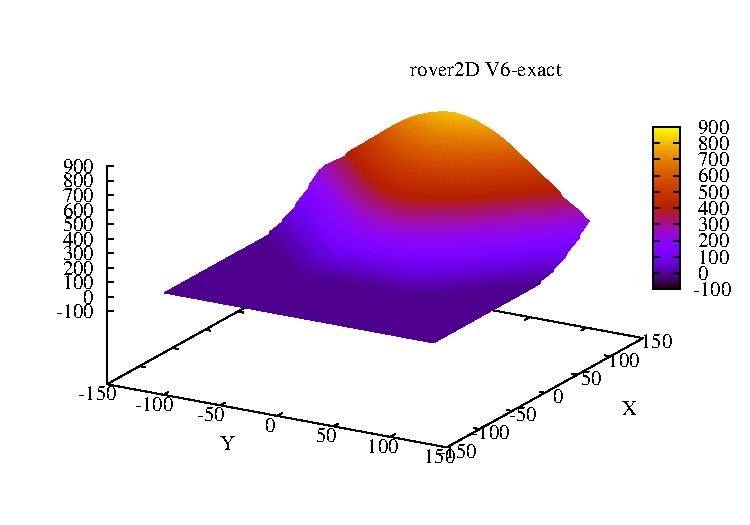
\includegraphics[width=0.45\textwidth, height=0.3\textwidth]{Figures/rover2D/rover2dV6-0.pdf}
	 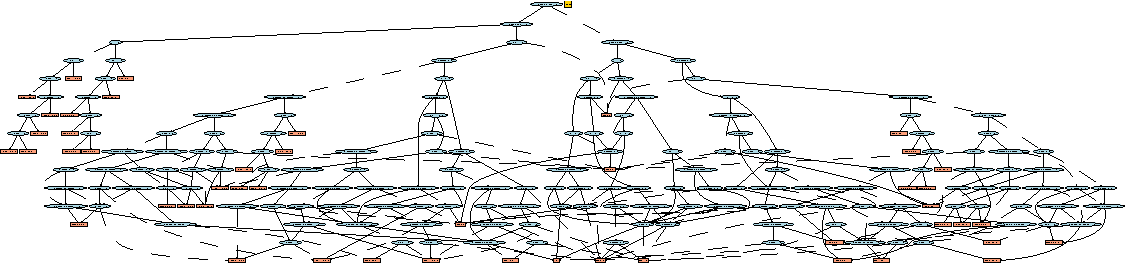
\includegraphics[width=0.45\textwidth, height=0.3\textwidth]{Figures/rover2D/rover2dV6-0xadd.pdf}
	 \label{V6-0xadd}
}
\subfigure[Value at $6^{th}$ iteration for $5\%$ approximate SDP.] {
	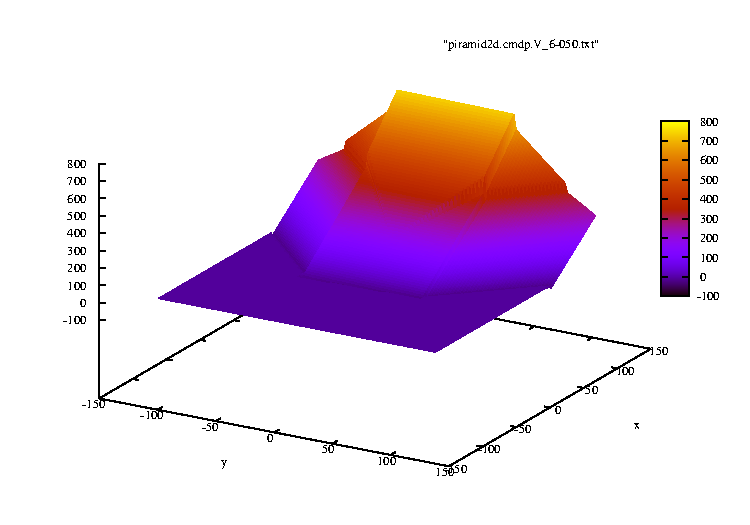
\includegraphics[width=0.45\textwidth, height=0.3\textwidth]{Figures/rover2D/rover2dV6-5.pdf}
	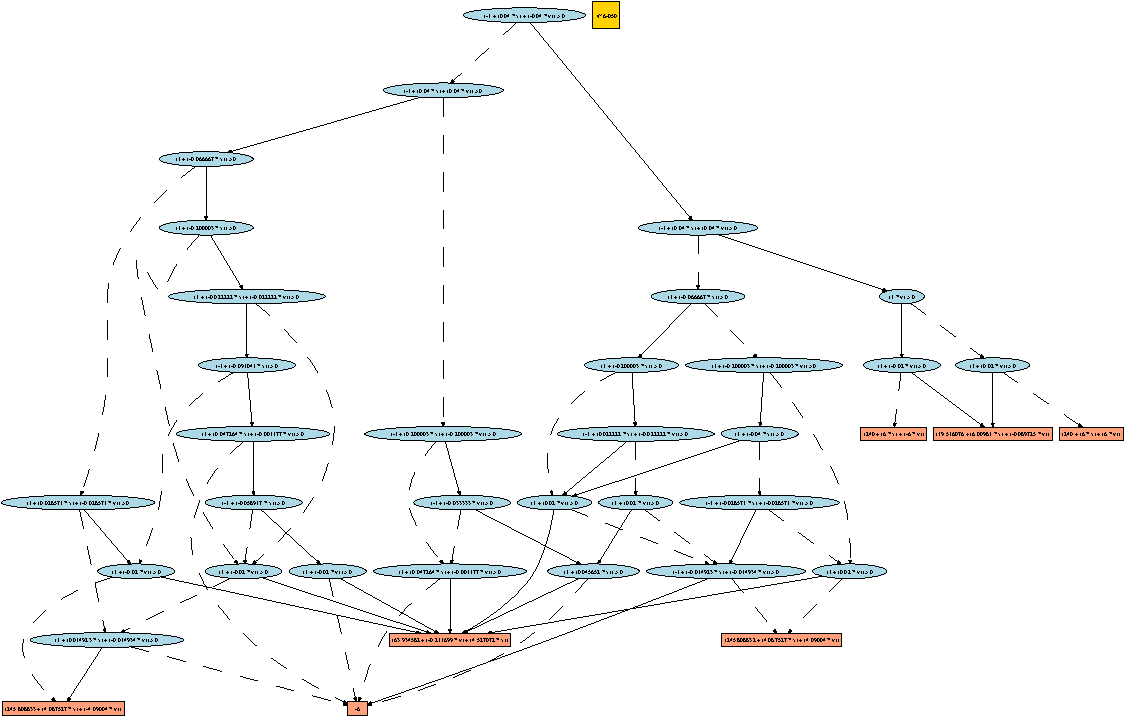
\includegraphics[width=0.45\textwidth, height=0.3\textwidth]{Figures/rover2D/rover2dV6-5xadd.pdf}
	 \label{V6-5xadd}
}
\caption {\footnotesize
	Value function at iteration 6 for the \MarsRoverBi domain;
	{\it (top)} Exact value function; 	{\it (bottom)} Approximate value function with error bounded 5\% per iteration;
	{\it (left)} 3D Plots; {\it (right)} XADD Diagrams.
}
\label{fig:Mars2DV6}
\vspace{-5mm}
\end{figure*}

\begin{figure*}[tbph!]
\centering
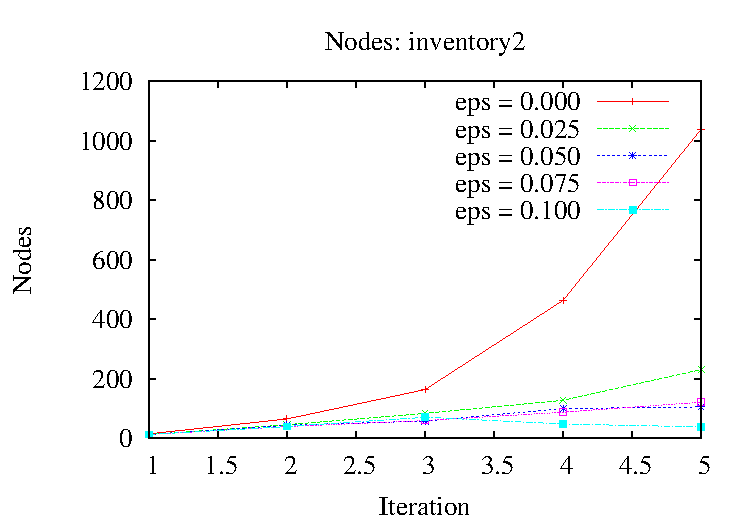
\includegraphics[width=0.32\textwidth]{Figures/inventory/inventory2Nodes.pdf}
\hspace{1mm}
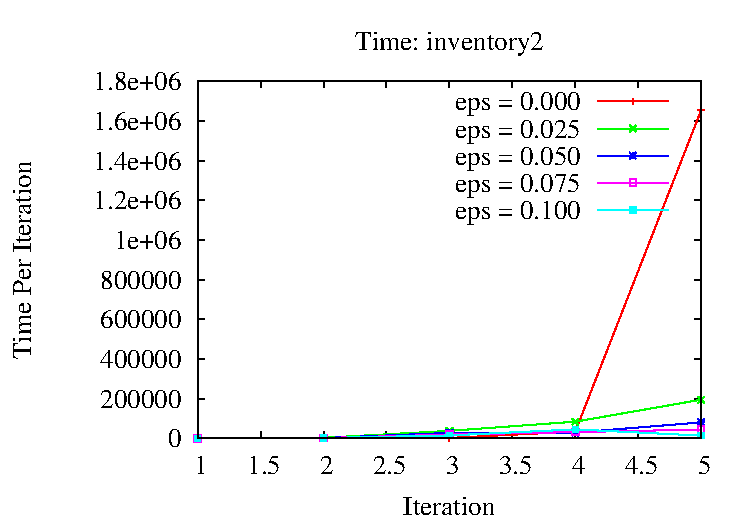
\includegraphics[width=0.32\textwidth]{Figures/inventory/inventory2Time.pdf}
\hspace{1mm}
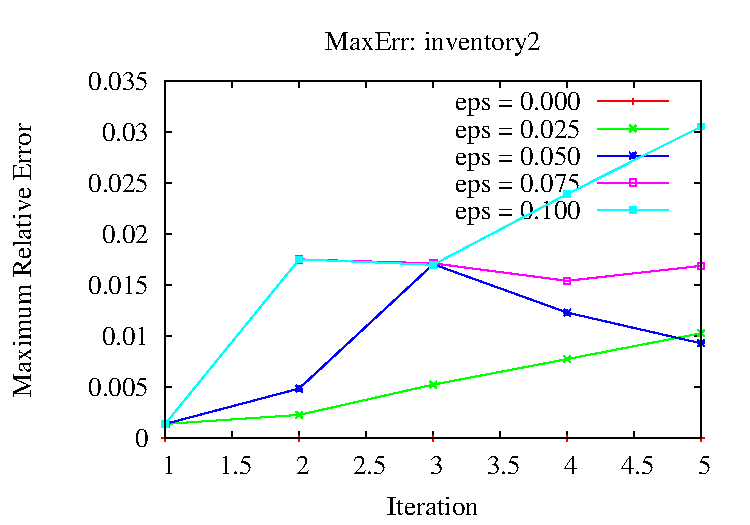
\includegraphics[width=0.32\textwidth]{Figures/inventory/inventory2MaxErr.pdf}
\\
\vspace{5mm}
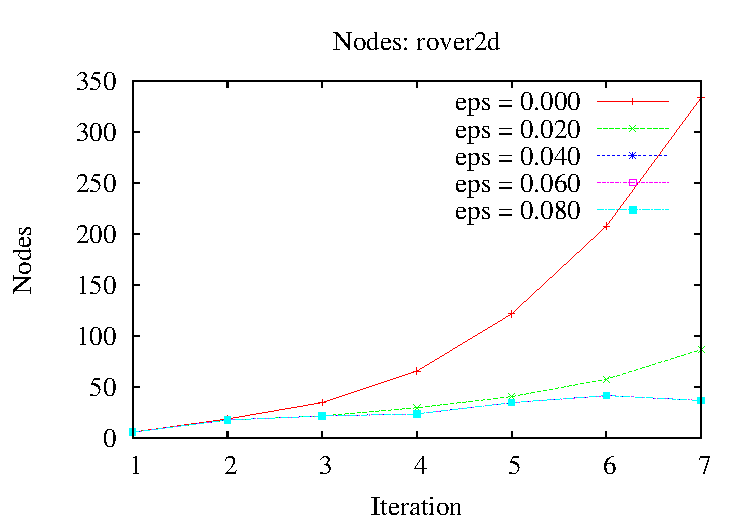
\includegraphics[width=0.32\textwidth]{Figures/rover2D/rover2d-Nodes.pdf}
\hspace{1mm}
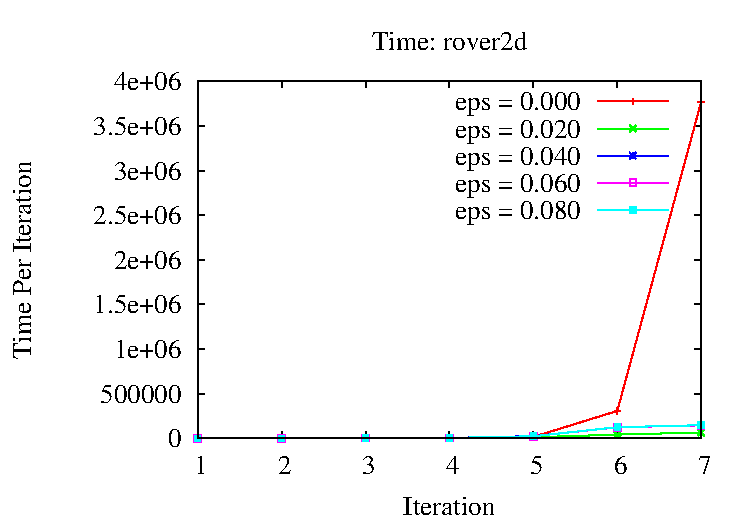
\includegraphics[width=0.32\textwidth]{Figures/rover2D/rover2d-Time.pdf}
\hspace{1mm}
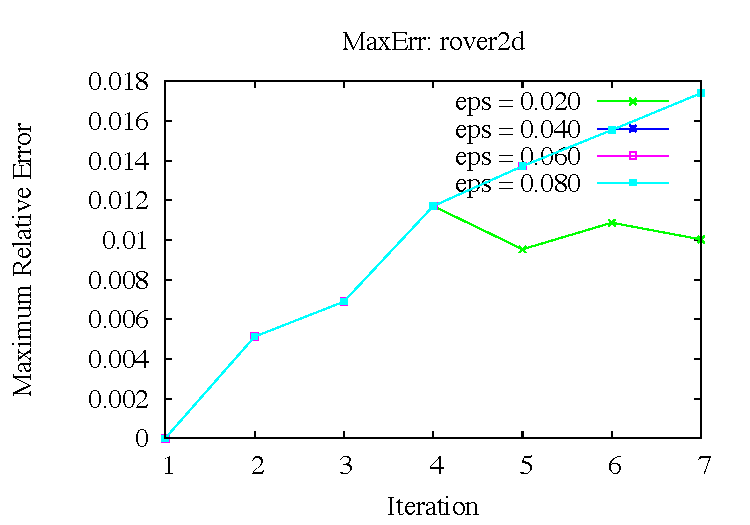
\includegraphics[width=0.32\textwidth]{Figures/rover2D/rover2d-MaxErr.pdf}
\caption{\footnotesize Performance plots for $\MarsRoverBi$ and $\Invent$2 with 5 different relative errors (eps):
{\it (left)}  Space (number of Nodes);
{\it (middle)} Time (miliseconds);
{\it (right)} Maximal error as fraction of the max value.
}
\label{fig:Value}
\vspace{-5mm}
\end{figure*}

In Figure~\ref{fig:Mars2DV6}, we can clearly see the effect of compression. In the 3D plots, a much simpler surface is obtained for the 5\% error compression, and correspondingly, in the diagrams, the number of nodes is greatly reduced, which enables a much faster computation of XADD operations and bounded error solution. 

\Invent:
In this domain, there are $n$ continuous resources that can be bought and sold. There are $n$ non-parametric actions $order$-$i$ for each resource, $ 1 \leq i \leq n$. The maximum amount of  each resource that is sold on one iteration depends on a stochastic demand variable $d$ that is true with $60\%$ probability. The resource $x_i'$ for action $order$-$i$ is given by:

\vspace{-8mm}
{\footnotesize
\begin{align*}
x_i' & = \begin{cases} 
(d') \wedge (x_i > 150) &: x_i + 200 - 150\\
(d') \wedge (x_i < 150) &:  200\\
(\neg d') \wedge (x_i > 50) &: x_i + 200 - 50\\
(\neg d') \wedge (x_i < 50) &:  200\\
\end{cases} \\
\end{align*} }
\vspace{-14mm}

and for other resources $x_j'$, $1 \leq j \leq n$, $j\neq i$:\\

\vspace{-10mm}
{\footnotesize
\begin{align*}
x_j' & = \begin{cases} 
(d') \wedge (x_j > 150) &: x_j - 150\\
(d') \wedge (x_j < 150) &:  0\\
(\neg d') \wedge (x_j > 50) &: x_j - 50\\
(\neg d') \wedge (x_j < 50) &:  0\\
\end{cases} \\
R & = \sum_{k} {x_k' - x_k}\\
\end{align*} }
\vspace{-6mm}

Figure \ref{fig:Value} shows the results of exact and approximate
solutions for two domains. In the left plots we notice how the
approximation does compress the XADD significantly. The remaining
plots, show that the compression results in faster computation while
never exceeding the allowed error.
